\documentclass[tikz,border=5pt]{standalone}
\usepackage{amsmath}
\usetikzlibrary{calc,arrows.meta,decorations.markings}
\definecolor{old}{RGB}{40,80,165}
\definecolor{star}{RGB}{195,80,15}
\definecolor{merged}{RGB}{110,55,150}
\tikzset{dot/.style={circle,fill=black,inner sep=1.5pt},flow/.style={postaction={decorate},decoration={markings,mark=at position .76 with {\arrow{Stealth}}}}}
\newcommand{\res}[3]{%
 \draw[#3,line width=.7pt,flow] (#1)--(#2);
 \path (#1)--(#2) node[midway,sloped,draw=#3,fill=white,minimum width=5mm,minimum height=1.7mm,inner sep=0pt,rotate=0]{};}
\begin{document}
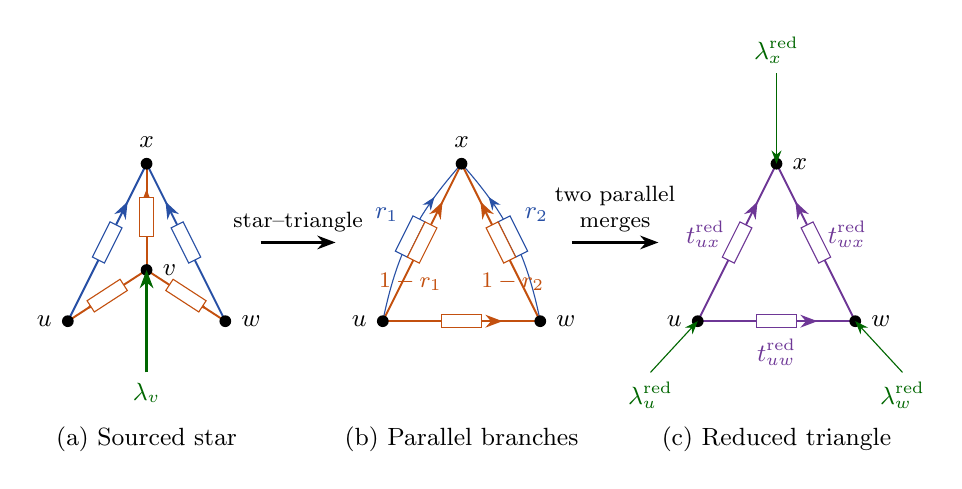
\begin{tikzpicture}[x=1cm,y=1cm,font=\small]
\begin{scope}
 \coordinate(u) at (0,0);\coordinate(w) at (2,0);\coordinate(x) at (1,2);\coordinate(v) at (1,.65);
 \node at (1,-1.5){(a) Sourced star};
 \res{u}{x}{old}\res{w}{x}{old}\res{v}{u}{star}\res{v}{w}{star}\res{v}{x}{star}
 \foreach \p/\pos in {u/left,w/right,x/above,v/right}{\node[dot,label=\pos:$\p$] at (\p){};}
 \draw[-{Stealth},line width=.8pt,green!40!black] (1,-.65)--(v) node[pos=0,below] {$\lambda_v$};
\end{scope}
\draw[-{Stealth},thick] (2.45,1)--(3.4,1) node[midway,above,align=center,font=\footnotesize]{star--triangle};
\begin{scope}[xshift=4cm]
 \coordinate(u) at (0,0);\coordinate(w) at (2,0);\coordinate(x) at (1,2);
 \node at (1,-1.5){(b) Parallel branches};
 \draw[old,flow] (u) to[bend left=15] (x);
 \path (u) to[bend left=15] node[midway,sloped,draw=old,fill=white,minimum width=5mm,minimum height=1.7mm,inner sep=0pt]{} (x);
 \draw[old,flow] (w) to[bend right=15] (x);
 \path (w) to[bend right=15] node[midway,sloped,draw=old,fill=white,minimum width=5mm,minimum height=1.7mm,inner sep=0pt]{} (x);
 \res{u}{x}{star}\res{w}{x}{star}\res{u}{w}{star}
 \node[old] at (.05,1.35){$r_1$};\node[old] at (1.95,1.35){$r_2$};
 \node[star,font=\footnotesize] at (.35,.5){$1-r_1$};\node[star,font=\footnotesize] at (1.65,.5){$1-r_2$};
 \foreach \p/\pos in {u/left,w/right,x/above}{\node[dot,label=\pos:$\p$] at (\p){};}
\end{scope}
\draw[-{Stealth},thick] (6.4,1)--(7.5,1) node[midway,above,align=center,font=\footnotesize]{two parallel\\merges};
\begin{scope}[xshift=8cm]
 \coordinate(u) at (0,0);\coordinate(w) at (2,0);\coordinate(x) at (1,2);
 \node at (1,-1.5){(c) Reduced triangle};
 \res{u}{x}{merged}\res{w}{x}{merged}\res{u}{w}{merged}
 \node[merged] at (.1,1.1){$t_{ux}^{\mathrm{red}}$};\node[merged] at (1.9,1.1){$t_{wx}^{\mathrm{red}}$};\node[merged] at (1,-.4){$t_{uw}^{\mathrm{red}}$};
 \foreach \p/\pos in {u/left,w/right,x/right}{\node[dot,label=\pos:$\p$] at (\p){};}
\draw[-{Stealth},green!40!black] (-.6,-.65)--(u) node[pos=0,below] {$\lambda_u^{\mathrm{red}}$};
 \draw[-{Stealth},green!40!black] (2.6,-.65)--(w) node[pos=0,below] {$\lambda_w^{\mathrm{red}}$};
 \draw[-{Stealth},green!40!black] (1,3.15)--(x) node[pos=0,above] {$\lambda_x^{\mathrm{red}}$};
\end{scope}
\end{tikzpicture}
\end{document}
